% command to draw a cube, used as illustration in chapter on functions
\newcommand{\drawCube}[4]{
	% first argument: ll position
	% second argument: x shift
	% 3rd argument: # of arguments
	% 4th argument: size (default = 1)
	% define cube coordinates
	\coordinate (A#1) at (#2,    0,     0);
	\coordinate (B#1) at ({#2+#4},0,     0);
	\coordinate (C#1) at ({#2+#4},#4,0);
	\coordinate (D#1) at (#2,    #4,0);
	\coordinate (E#1) at (#2,     0,#4);
	\coordinate (F#1) at ({#2+#4}, 0,#4);
	\coordinate (G#1) at ({#2+#4},#4,#4);
	\coordinate (H#1) at (#2,    #4,#4);

	% draw cube
	\draw[thick] (A#1) -- (B#1) -- (C#1) -- (D#1) -- cycle;
	\draw[thick] (E#1) -- (F#1) -- (G#1) -- (H#1) -- cycle;
	\draw[thick] (A#1) -- (E#1);
	\draw[thick] (B#1) -- (F#1);
	\draw[thick] (C#1) -- (G#1);
	\draw[thick] (D#1) -- (H#1);

	% define lower left corner of doors
	% door with is defined to always be 0.2*size wide and 0.5*size high. We also define that the space between each door is the remaining width,
	% i.e., if we have three doors, then the remaining space is (size-0.2*size*3)/(3+1)

	% calculate how much empty space to leave between each door
	\pgfmathsetmacro\emptyspace{(#4-0.2*#4*#3)/(#3+1)}

	% define amount of space per door
	\pgfmathsetmacro\doorsspace{0.2*#4}

	\foreach \x in {1,...,#3} {
			\pgfmathsetmacro\llCord{\emptyspace*\x+\doorsspace*(\x-1)}
			% lower door coordinate
			\coordinate (llD\x#1) at ({\llCord+#2},0,#4);

			% draw doors
			\fill[blue!50, rounded corners] (llD\x#1) -- ++(0,{#4/2},0) -- ++({0.2*#4},0,0)node[pos=.5, below](in#1\x){\textcolor{blue}{\texttt{x\x}}} -- ++(0,{-#4/2},0);

			% lower door coordinate for value (for later annotation)
			\coordinate (llD\x#1val) at ({\llCord-.1*#4+#2},{-.2*#4},#4); % the coordinate is simple .1*size to the left of the ll corner and .2*size below.
		}

	% coordinate for result door
	\coordinate (llDOut#1) at ({#2+#4},0,{#4*.2});
	\fill[green!50, rounded corners] (llDOut#1) -- ++(0,{#4/2},0) -- ++(0,0,{#4/2})node[pos=0.8,rotate=45, below, align=center](out#1){\textcolor{black}{\tiny\texttt{out#1}\normalsize}} -- ++(0,{-#4/2},0);

	% draw a 2D rectangle around the cube
	\node[fit=(E#1) (C#1), inner sep=4pt, red, dotted, draw, line width=1pt,rounded corners](dottedRect#1) {};
	% annotate the two-d rect
	\node[above=5pt of dottedRect#1.north west, anchor=west, align=left]{\textcolor{red}{\texttt{def a#1(\textcolor{blue}{\foreach\x in {1,...,#3}{x\x, }...})}\normalsize}};
}


\begin{frame}
    \centering
    \begin{figure}[H]
        
\includegraphics[keepaspectratio, width=0.7\paperwidth, height=\paperheight]{LeeLogo}
    \end{figure}
    Informatik: Programmieren\\
    \emoji{cook} Kapitel 7: \textbf{Funktionen mit \tjinline{return}}
\end{frame}

\begin{frame}
    \begin{figure}[H]
        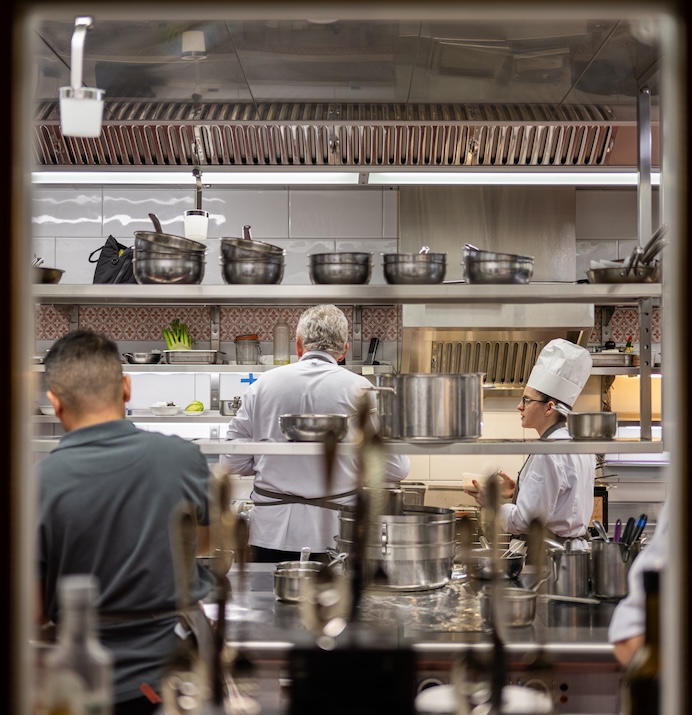
\includegraphics[keepaspectratio, width=.6\linewidth]{GrundlagenInfo/00_Programmieren/Figures/cook}
    \end{figure}
    \begin{center}
    Woran erinnert Sie dieses Bild?
    \end{center}
\end{frame}

\begin{frame}[fragile]{Funktionen}
\begin{centering}
\only<1->{Womit können Funktionen verglichen werden?}\only<2->{ Weshalb?}
\end{centering}
\only<3->{
\begin{columns}
\begin{column}{.5\linewidth}
\begin{figure}
\centering
\includegraphics[width=\columnwidth]{"GrundlagenInfo/00_Programmieren/Figures/Fine Dining 1"}\\[.6cm]
\includegraphics[width=\columnwidth]{"GrundlagenInfo/00_Programmieren/Figures/Fine Dining 2"}
\end{figure}

\end{column}

\begin{column}{.5\linewidth}
\begin{figure}
\centering
\includegraphics[width=\columnwidth]{"GrundlagenInfo/00_Programmieren/Figures/Fine Dining 3"}\\[.6cm]
\includegraphics[width=\columnwidth]{"GrundlagenInfo/00_Programmieren/Figures/Fine Dining 4"}
\end{figure}
\end{column}
\end{columns}
}
\end{frame}

\begin{frame}[fragile]{Funktionierende Funktion? \emoji{bug}}
\begin{lstlisting}
def summiere(x1, x2):
    summe = x1 + x2
    
summiere(3, 5)
print(summe)
\end{lstlisting}
\begin{center}
Funktioniert dieser Code? 

Wenn ja, was gibt er aus? Wenn nein, weshalb nicht?
\end{center}
\end{frame}

\begin{frame}[fragile]{Funktionen}{Grundidee}
\begin{figure}[H]
% Use the \drawCube macro to draw various cubes
\centering
\resizebox{.7\linewidth}{!}{
\begin{tikzpicture}
\drawCube{1}{0}{2}{3}
\node[fill=blue!50, rounded corners] (input1) at (llD11val){3};
\node[fill=blue!50, rounded corners] (input2) at (llD21val){12};
\draw[thick,->] (input1) -- (in11);
\draw[thick,->] (input2) -- (in12);
\node[fill=green!50, rounded corners](outVal1) at (5,-.6,3){36};
\draw[thick,->] (out1) -- (outVal1);

\node[fill=red!50, rounded corners](outVal1) at (1.5,1.5,1.5){\emoji{cook}};
\end{tikzpicture}
}
\end{figure}
\end{frame}

\begin{frame}[fragile]{Funktionen: Mit \lstinline|return|}
\begin{lstlisting}
def summiere(x1, x2):
    summe = x1 + x2
    return (*@\colorbox{CornflowerBlue!80}{sum\tikzmark{arrowFromEx01}me}@*)
    


(*@\colorbox{CornflowerBlue!80}{r\tikzmark{arrowToEx01}es}@*) = summiere(3, 5)
print(res)
\end{lstlisting}
\begin{tikzpicture}[overlay,remember picture]
   % Wert zurückgeben
	\draw[red,-stealth] (arrowFromEx01.north) to[bend left] node[align=left, pos=.3, right, fill=RoyalBlue,fill opacity=.5, text opacity=1, text=black,rounded corners] {Wert an das Hauptprogramm zurückgeben \\\textit{und} Variable speichern, z.B. \lstinline|res|} (arrowToEx01);
\end{tikzpicture}
\end{frame}

\begin{frame}[fragile]{Aufträge}
Im Skript ``Funktionen'', auf Moodle (Programmier-Kurs):
\begin{itemize}
\item \abgabebox{Aufgaben 1.4 - 1.7 (Abgabe auf Moodle)}
\item \aufgabebox{Aufgabe 1.8}
\end{itemize}
\end{frame}

\begin{frame}{Fazit}
\begin{itemize}[<+->]
	\item \emoji{thumbs-up} Vorteil von \tjinline{return}-Werten: man kann nun das Resultat einer Funktion in einer Variable speichern und \textbf{weiterverwenden}
	\item \emoji{thumbs-up} Vorteil von Funktionen: Code wird \textbf{modular}
	\item Funktionen sind Definitionen...
	\item \emoji{clipboard} ...die wie ein \textbf{Kochrezept} funktionieren:
	\begin{itemize}
		\item \emoji{bread} \emoji{cheese} \emoji{poultry-leg} Gewisse Inputs, bzw. \textbf{Parameter} können akzeptiert werden (müssen aber nicht)
		\item \emoji{hamburger} Gewisse Outputs, bzw. \textbf{Return-Werte }können zurückgeben werden (müssen aber nicht)
	\end{itemize}
	\item \emoji{cook} ...die wie ein \textbf{Koch} funktionieren (\textbf{Modularität}):
	\begin{itemize}
		\item Ein Koch schneidet alle Gemüse...
		\item ..., ein Koch grilliert die Gemüse...
		\item ..., ein Koch bereitet die Teller schön zu...
		\item etc. (jeder Koch ist eine \tjinline{def})
	\end{itemize}
\end{itemize}
\end{frame}